\section{Performances}
\label{surface_reconstruction_section_performances}

We provide some performance numbers for scanning data. We measure the Poisson implicit function computation time, the contouring time for a range of approximation distances, the memory occupancy as well as the influence of the point set simplification. The machine used is a PC running Linux 32 bits with an Intel CPU Core 2 processor clocked at 3 GHz and with 3 GB of RAM. The software is compiled with g++ 4.3.1 compiler with the 03 option which maximizes speed.  All measurements were done using the \ccThirdPartyTaucs\ library even if we now recommend to use the \ccThirdPartyEigen\ library.

\subsection{Poisson implicit function}

The point set chosen for benchmarking the Poisson implicit function is the Bimba con Nastrino point set (1.6 million points) depicted by Figure~\ref{Surface_reconstruction_points_3-fig-poisson_bench}. We measure the Poisson implicit function computation (i.e., the call to \ccc{Poisson_reconstruction_function::compute_implicit_function()} denoted by Poisson solve hereafter) for this point set as well as for simplified versions obtained through random simplification. The following table provides Poisson solve computation times in seconds for an increasing number of points.

\begin{tabular}{|c|c|}
  \hline
  Number of points (x1000) & Poisson solve duration (in s) \\
  \hline
  60                         & 65 \\
  120                        & 137 \\
  250                        & 282 \\
  500                        & 566 \\
  1,000                       & 1,130 \\
  1,500                       & 1,777 \\
  1,600                       & 1,919 \\
  \hline
\end{tabular}

% Insert image poisson_bench.jpg/.eps
\begin{center}
    \begin{ccTexOnly}
        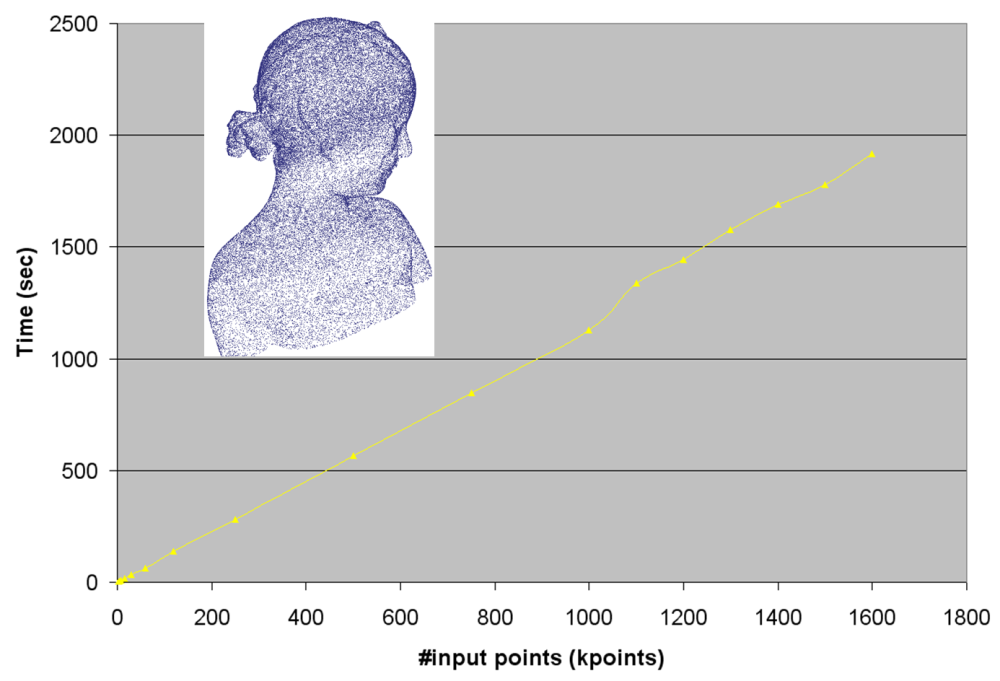
\includegraphics[width=1.0\textwidth]{Surface_reconstruction_points_3/poisson_bench}
    \end{ccTexOnly}
    \begin{ccHtmlOnly}
        <img style="max-width: 100%;" border=0 src="./poisson_bench.jpg"><P>
    \end{ccHtmlOnly}
    \begin{figure}[h]
        \caption{Poisson implicit function computation duration (in s)
                 against the number of points  for the Bimba con Nastrino
                 point set with 1.6M points (shown)
                 as well as for simplified versions.}
        \label{Surface_reconstruction_points_3-fig-poisson_bench}
    \end{figure}
\end{center}



\subsection{Contouring}

The point set chosen for benchmarking the contouring stage is the Bimba con Nastrino point set simplified to 120k points. We measure the contouring (i.e. the call to \ccc{make_surface_mesh()}) duration and the reconstruction error for a range of approximation distances.
The reconstruction error is expressed as the average distance from input points to the reconstructed surface in mm (the Bimba con Nastrino statue is 324 mm tall).

\begin{tabular}{|c|c|c|}
  \hline
  Approx. distance (*average spacing)    & Contouring duration (in s) & Reconstruction error (mm) \\
  \hline
  0.1                                    & 177                       & 0.13 \\
  0.25                                   & 47                        & 0.155 \\
  0.5                                    & 21                        & 0.23 \\
  1                                      & 10                        & 0.4 \\
  2                                      & 5                         & 0.78 \\
  \hline
\end{tabular}

% Insert image contouring_bench.jpg/.eps
\begin{center}
    \begin{ccTexOnly}
      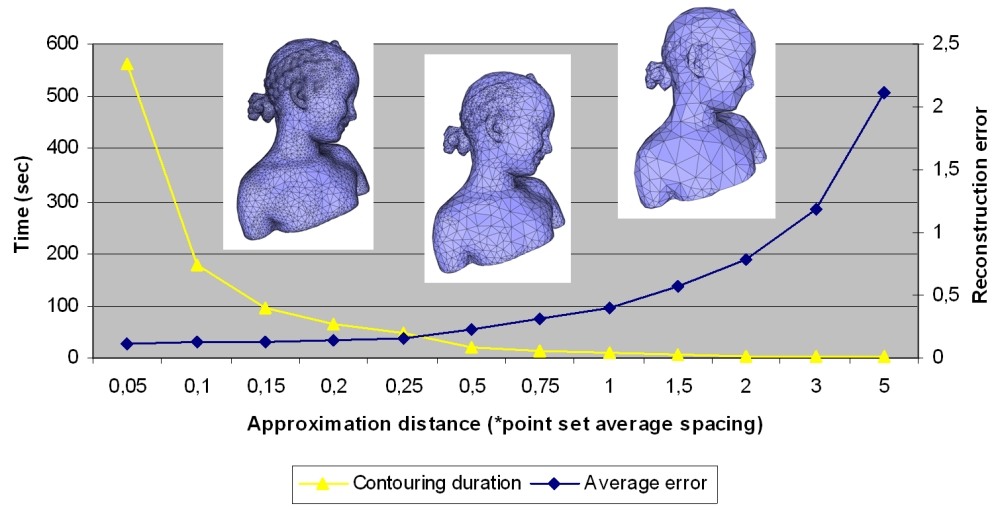
\includegraphics[width=1.0\textwidth]{Surface_reconstruction_points_3/contouring_bench}
    \end{ccTexOnly}
    \begin{ccHtmlOnly}
        <img style="max-width: 100%;" border=0 src="./contouring_bench.jpg"><P>
    \end{ccHtmlOnly}
    \begin{figure}[h]
        \caption{Contouring duration (in s) and reconstruction error (mm)
                 against several approximation distance parameters
                 for the Bimba con Nastrino point set simplified to 120k points.}
        \label{Surface_reconstruction_points_3-fig-contouring_bench}
    \end{figure}
\end{center}



\subsection{Memory}

We measure the memory occupancy for the reconstruction of the full Bimba con Nastrino point set (3.8 millions points) as well as for simplified versions.\\
The Poisson implicit function computation has a memory peak when solving the Poisson linear system using the {\sc Taucs} sparse linear solver. For large point sets, it may fail to allocate big chunks of memory due to memory fragmentation.\\
The exact limit depends of the allocation scheme used by the compiler. In our experiments, a PC running Linux 32 bits can reconstruct the Bimba con Nastrino point set up to 1.6M points while Windows 32 bits is limited to 1.3M points.\\

\begin{tabular}{|c|c|}
  \hline
  Number of points (x1000) & Memory occupancy (MBytes) \\
  \hline
  60                         & 330 \\
  120                        & 660 \\
  250                        & 630 \\
  500                        & 980 \\
  1000                       & 1570 \\
  1200                       & 1939 \\
  \hline
\end{tabular}

% Insert image memory_bench.jpg/.eps
\begin{center}
    \begin{ccTexOnly}
        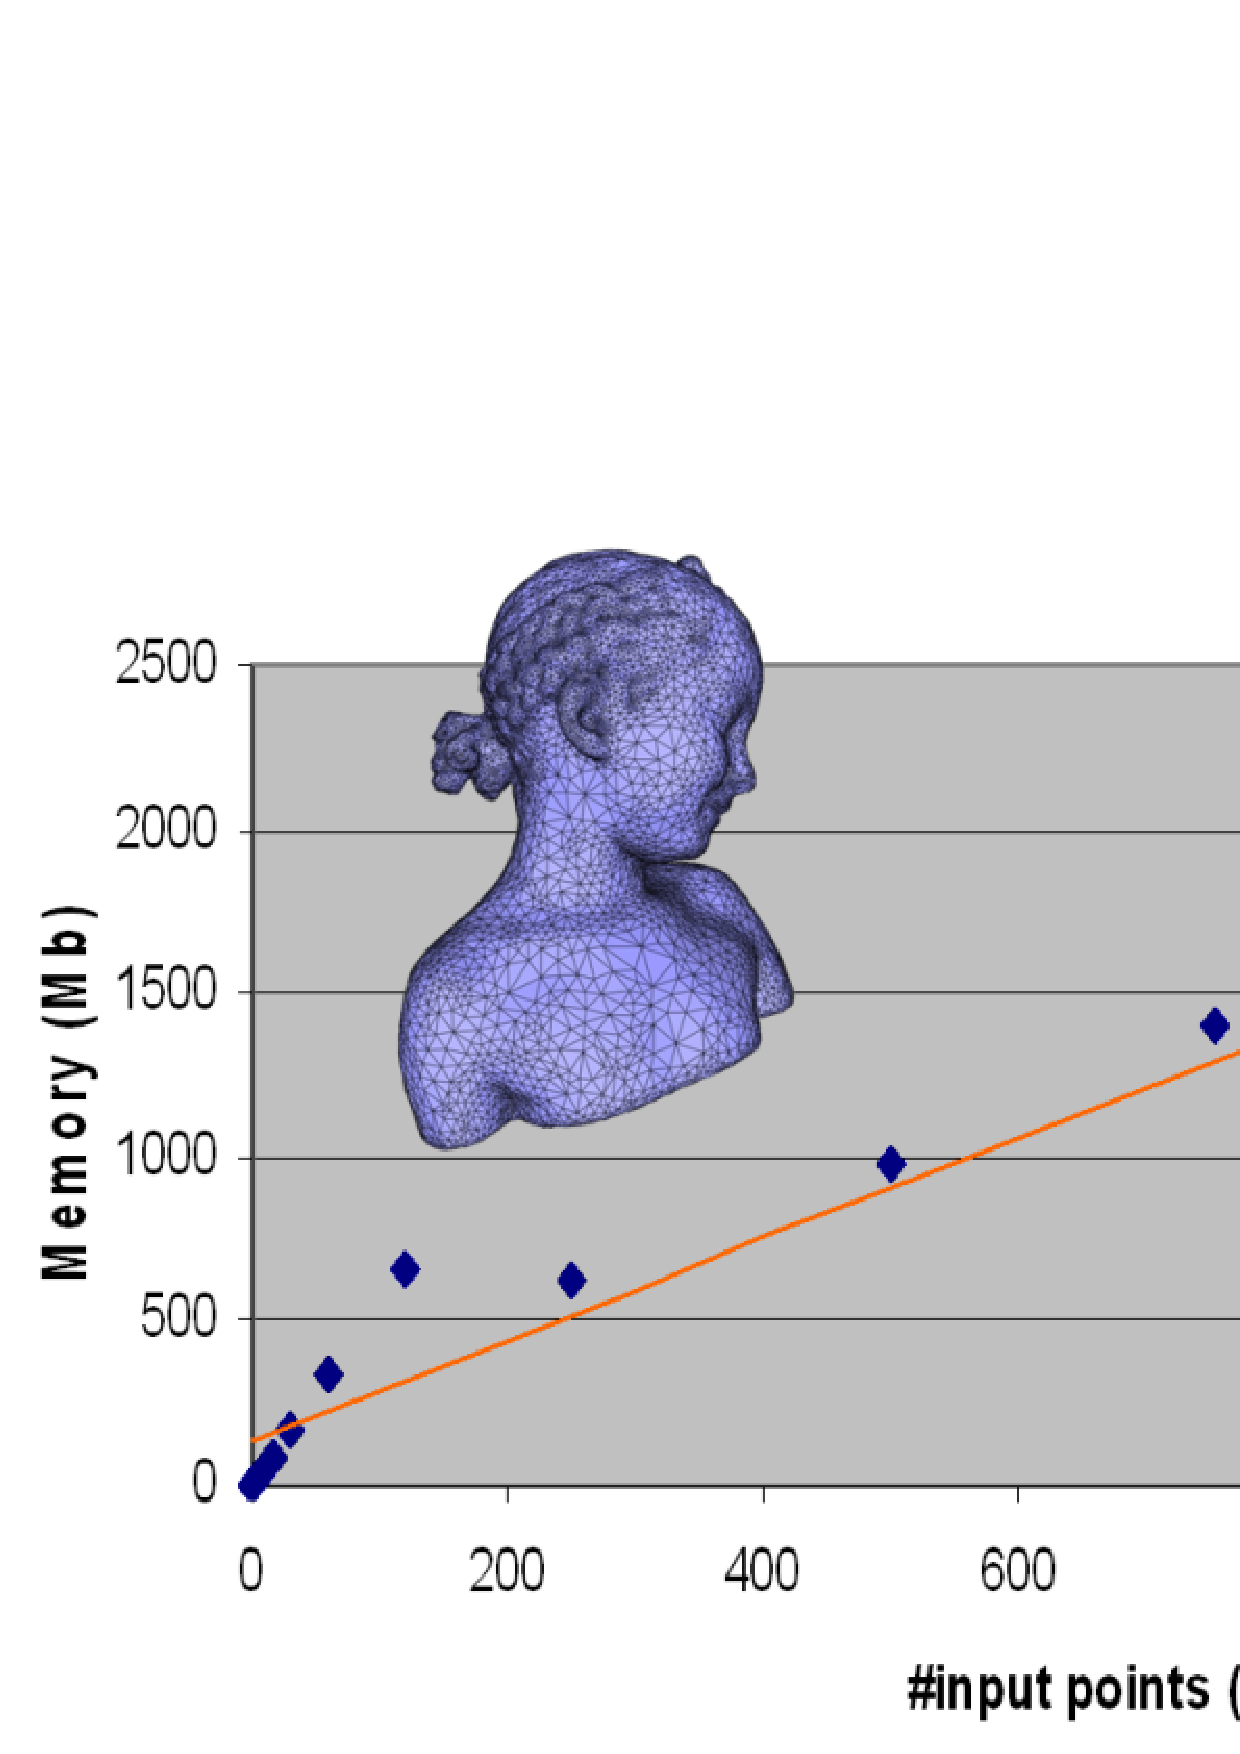
\includegraphics[width=1.0\textwidth]{Surface_reconstruction_points_3/memory_bench}
    \end{ccTexOnly}
    \begin{ccHtmlOnly}
        <img style="max-width: 100%;" border=0 src="./memory_bench.jpg"><P>
    \end{ccHtmlOnly}
    \begin{figure}[h]
        \caption{Memory occupancy (in MBytes) against number of points
                 for the Bimba con Nastrino point set with 1.2M points
                 as well as for simplified versions.
                 The best fitting line is shown.}
        \label{Surface_reconstruction_points_3-fig-memory_bench}
    \end{figure}
\end{center}



\subsection{Point Set Simplification}

Due to the memory limitations described above, we recommend to simplify the point sets captured by laser scanners.\\
We measure the reconstruction error for the Bimba con Nastrino point set (1.6M points) as well as for simplified versions. All reconstructions use the recommended contouring parameter approximation distance = 0.25 * the input point set's average spacing.
The reconstruction error is expressed as the average distance from input points to the reconstructed surface in mm (the Bimba con Nastrino statue is 324 mm tall).

\begin{tabular}{|c|c|}
  \hline
  Number of points (x1000) & Reconstruction error (mm) \\
  \hline
  60                         & 0.27 \\
  120                        & 0.15 \\
  250                        & 0.11 \\
  500                        & 0.079 \\
  1,000                       & 0.066 \\
  1,500                       & 0.061 \\
  1,600                       & 0.06 \\
  \hline
\end{tabular}

% Insert image simplification_bench.jpg/.eps
\begin{center}
    \begin{ccTexOnly}
        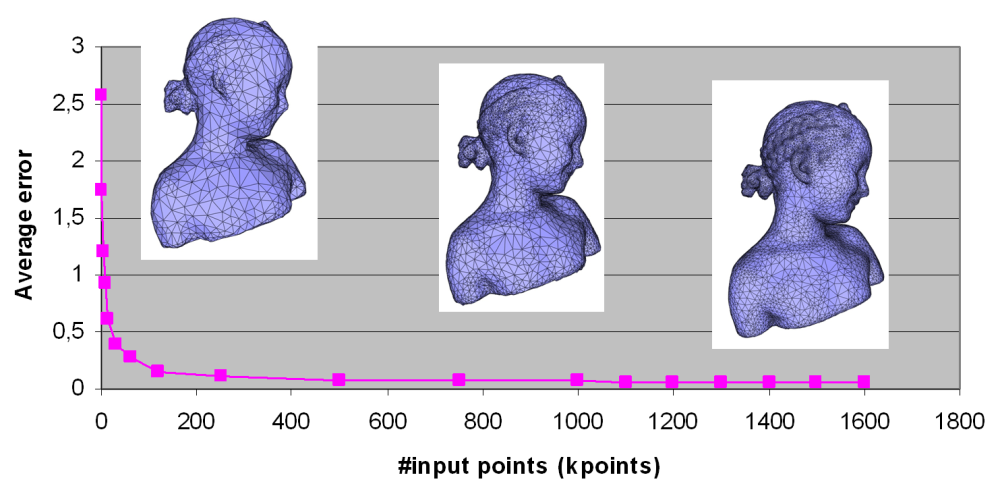
\includegraphics[width=1.0\textwidth]{Surface_reconstruction_points_3/simplification_bench}
    \end{ccTexOnly}
    \begin{ccHtmlOnly}
        <img style="max-width: 100%;" border=0 src="./simplification_bench.jpg"><P>
    \end{ccHtmlOnly}
    \begin{figure}[h]
        \caption{Reconstruction error (mm) against number of points
                 for the Bimba con Nastrino point set with 1.6M points
                 as well as for simplified versions.}
        \label{Surface_reconstruction_points_3-fig-simplification_bench}
    \end{figure}
\end{center}





